% week11_thu_pair_reasoning.tex -- DSCT Week 11 Thursday, Oct 29 2026.
% Sources: week-11/instructor/thursday-run-of-show.md, week-11/README.md,
% assignments/pair-reasoning-report.md (six-field scaffold), lessons/09-relations.md.
% Every number below is reproduced by scripts/verify_week11_thu_pair_reasoning.py.
\documentclass[aspectratio=169,10pt]{beamer}
\usetheme{Madrid}
\usepackage{tikz}
\usepackage{amssymb}
\title{Your Partner Is the Test Suite}
\subtitle{Week 11 Thursday --- Pair Reasoning: classify a relation under challenge}
\author{COMSC 2043 \textbullet\ Discrete Structures and Critical Thinking}
\date{October 29, 2026}
\begin{document}

\frame{\titlepage
\note{Run of show (75 min of class; the table in thursday-run-of-show.md adds up to 1:25, so plan to trim the last block if the room runs on a 75-minute clock). 0:00 starting position (10). 0:10 norms and the dice hook (8). 0:18 compare representations, worked classifier (27). 0:45 cross-pair challenge (13). 0:58 individual write-up and checkpoint time (14). 1:12 name the model limit, preview Week 12 (13). Theme: your partner's job is to break your claim with one pair; your job is to say what survived. No code required: a paper matrix is inspectable. Do not assign driver/navigator roles.}}

\begin{frame}{Today's destination}
\begin{itemize}
\item Put a classification in writing \textbf{before} you talk to anyone.
\item Compare representations (pairs, matrix, digraph) and hunt for the \textbf{one pair} that separates two positions.
\item Challenge another pair's claim with evidence, not volume.
\item Say what changed, what survived, and where the model stops being true.
\end{itemize}
\note{Say it plainly: Pair Reasoning is not collaboration to split the work and not a debate to win. It is exposing your reasoning to someone who will push on it. If two partners already agree, the task is to test whether the agreement deserves confidence. Today's evidence is your reasoning before, during, and after the challenge.}
\end{frame}

\begin{frame}{Solo first (10 min): classify this relation}
Let $S=\{1,2,3,4\}$ and
\[R=\{(1,1),(2,2),(3,3),(4,4),(1,2),(2,1),(2,3),(3,2)\}.\]
On your own paper, \textbf{before talking}: for each of reflexive, symmetric, antisymmetric, transitive write \emph{yes} or \emph{no}, one line of why, and a confidence from 1 to 5. Then: equivalence, partial order, neither, or both?
\vspace{4pt}

\textbf{Do not look at a neighbor's paper.} Wrong answers recorded now are worth more than right answers copied later.
\note{This is the individual starting position from the Pair Reasoning contract. Walk the room, do not correct anyone. Answers to hold back (do not reveal yet): reflexive yes (all four loops). Symmetric yes: (1,2)/(2,1) and (2,3)/(3,2) are paired. Antisymmetric NO: (1,2) and (2,1) are both in R with 1 not equal 2. Transitive NO: (1,2) and (2,3) are in R but (1,3) is not. So it is neither an equivalence relation nor a partial order. Likely wrong answers: saying transitive because every pair has a partner; saying antisymmetric because symmetric ``feels opposite'' (symmetric and antisymmetric are not opposites). Collect confidence numbers: they pay off at 0:58. At the 10-minute mark say pencils down, then pair students.}
\end{frame}

\begin{frame}{Pairing norms (what is and is not allowed)}
\begin{columns}[T]
\begin{column}{0.48\textwidth}
\textbf{Do}
\begin{itemize}
\item Compare definitions and assumptions first.
\item Name the \emph{strongest} part of your partner's reasoning.
\item Challenge with a pair, a chain, or a definition.
\item Separate ``the AI said'' from ``we checked.''
\end{itemize}
\end{column}
\begin{column}{0.48\textwidth}
\textbf{Do not}
\begin{itemize}
\item Split the work and merge answers.
\item Win by repeating louder.
\item Assume agreement means correct.
\item Copy a partner's write-up. It is yours alone.
\end{itemize}
\end{column}
\end{columns}
\vspace{6pt}
\textbf{Boundary:} Checkpoint 2 \emph{replaces} this week's Decision Gate. You submit one, not both.
\note{About 8 minutes including pairing. No driver/navigator roles; a paper matrix is fine, code is optional. Individual authorship matters: each person writes their own reflection and their own checkpoint. Quick check for understanding: ask ``if you and your partner agree, are you done?'' Expected: no, now test whether the agreement deserves confidence. Mention the three-way separation: the Odyssey checkpoint is the technical evidence; the pair reasoning is the social evidence; do not paste one into the other. Be neutral on what is submitted after class for the pairing itself and point to the Week 11 README; the old report category is retired from the graded course, so do not promise points for it.}
\end{frame}

\begin{frame}{Warm-up fight: pick a die}
Three dice, six faces each. You and your partner each pick one die; higher roll wins.
\begin{center}
\begin{tabular}{ll}
\textbf{A} & 2, 2, 4, 4, 9, 9 \\
\textbf{B} & 1, 1, 6, 6, 8, 8 \\
\textbf{C} & 3, 3, 5, 5, 7, 7 \\
\end{tabular}
\end{center}
\begin{enumerate}
\item Which die would you choose, and why? Argue it with your partner.
\item Define ``$X$ beats $Y$'' as: $X$ wins more often than $Y$. Is this relation \textbf{transitive}?
\end{enumerate}
\note{Hook. Let pairs fight for two minutes before revealing. Fun fact to say: all three dice have the same average, 5. So the usual instinct, ``higher average wins,'' gives no answer. The reveal is on the next slide. Teaching point: ``beats'' sounds like ``greater than,'' and greater-than is transitive, so students assume this is too. A name is a claim; the relation has to earn its label. This is the nontransitive dice of Efron, as used in probability puzzles. Do not claim a source beyond that; the face values here are computed in scripts/verify\_week11\_thu\_pair\_reasoning.py.}
\end{frame}

\begin{frame}{The dice relation, tested}
\begin{columns}[T]
\begin{column}{0.5\textwidth}
Each matchup has $6\times6=36$ outcomes:
\begin{center}
\begin{tabular}{lcc}
\textbf{Matchup} & \textbf{First wins} & \textbf{Chance} \\\hline
A vs B & 20 of 36 & 5/9 \\
B vs C & 20 of 36 & 5/9 \\
C vs A & 20 of 36 & 5/9 \\
\end{tabular}
\end{center}
No ties; every die has average 5.\\[4pt]
So A beats B, B beats C, \textbf{and C beats A}.
\end{column}
\begin{column}{0.46\textwidth}
\begin{center}
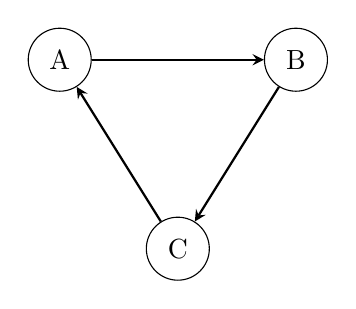
\begin{tikzpicture}[>=stealth,every node/.style={circle,draw,minimum size=8mm}]
\node (A) at (0,0) {A}; \node (B) at (3,0) {B}; \node (C) at (1.5,-2.4) {C};
\draw[->,thick] (A) -- (B); \draw[->,thick] (B) -- (C); \draw[->,thick] (C) -- (A);
\end{tikzpicture}
\end{center}
\end{column}
\end{columns}
\vspace{2pt}
Classify ``beats'': reflexive? symmetric? antisymmetric? transitive? Give the witness.
\note{Answers: not reflexive (a die does not beat itself); not symmetric (A beats B, B does not beat A); antisymmetric holds, but only vacuously, because there is no pair going both ways; not transitive: A beats B and B beats C, yet C beats A rather than A beats C. Witness chain: (A,B), (B,C) in R but (A,C) not in R. Whoever picks second wins: against any die there is a better reply, so the second chooser always has an edge (verified: every die has a die that beats it). Link back to Tuesday: rock-paper-scissors was the same cycle. Link forward: this is exactly why a prerequisite relation must not contain a cycle.}
\end{frame}

\begin{frame}{Same relation, three views: what each one makes easy}
\begin{center}
\begin{tabular}{lp{3.3cm}p{3.3cm}p{3.3cm}}
 & \textbf{Pair list} & \textbf{Matrix} & \textbf{Digraph} \\\hline
Reflexive & scan for $(a,a)$ & diagonal all 1s & loop on every node \\[3pt]
Symmetric & find each reverse & equals its mirror & every arrow has a return \\[3pt]
Antisymmetric & hunt two-way pairs & no mirrored off-diagonal 1s & no two-way arrows \\[3pt]
Transitive & chain, then look up & hardest to read & every two-step path has a shortcut \\
\end{tabular}
\end{center}
\vspace{4pt}
Disagree about a property? Switch representations and see whether the \textbf{answer stays the same}.
\note{Use this to run the 0:18 to 0:45 block: pairs compare their solo classifications, then redraw the relation in the representation they did NOT use. A disagreement that disappears in one view and survives in another means somebody mis-translated; that is the most common root cause. Typical translation errors: transposed matrix, reversed pair direction, missing loops. Matrix transitivity is the hardest to see by eye; the digraph is best for transitivity, the matrix is best for symmetry.}
\end{frame}

\begin{frame}{Worked example: the classifier trace}
\begin{columns}[T]
\begin{column}{0.4\textwidth}
Matrix of $R$ (row $a$, column $b$):
\[
\begin{array}{c|cccc}
 & 1&2&3&4\\\hline
1&1&1&0&0\\
2&1&1&1&0\\
3&0&1&1&0\\
4&0&0&0&1
\end{array}
\]
\end{column}
\begin{column}{0.58\textwidth}
\begin{tabular}{@{}lcp{4.2cm}@{}}
\textbf{Property} & & \textbf{Evidence} \\\hline
Reflexive & yes & diagonal all 1s \\
Symmetric & yes & matrix equals its mirror \\
Antisymmetric & \textbf{no} & $(1,2),(2,1)\in R$, $1\neq2$ \\
Transitive & \textbf{no} & $(1,2),(2,3)\in R$ but $(1,3)\notin R$ \\
\end{tabular}
\end{column}
\end{columns}
\vspace{6pt}
\textbf{Verdict:} neither an equivalence relation nor a partial order. It looks like ``is friends with'': reflexive and symmetric, but friend-of-a-friend breaks it.
\note{This is the instructor model: reveal answer to the solo problem. Say the claim and the witness in one sentence: ``R is not transitive, because (1,2) and (2,3) are in R and (1,3) is not.'' A second witness also exists: (3,2),(2,1) without (3,1). Ask: which one witness is enough? One is enough to say no. Note that two ``no''s means it is neither label, and that the reflexive-plus-symmetric prefix is what makes it feel like an equivalence relation.}
\end{frame}

\begin{frame}{Worked example: repair it, then name the bins}
\begin{itemize}
\item The two missing pairs are exactly $(1,3)$ and $(3,1)$. Add them: that is the \textbf{smallest} transitive fix.
\item New relation $R'$: reflexive $\checkmark$, symmetric $\checkmark$, transitive $\checkmark$, antisymmetric no.
\item So $R'$ is an \textbf{equivalence relation} with two bins: $\{1,2,3\}$ and $\{4\}$.
\end{itemize}
\begin{block}{Challenge move for your pair}
Take your own relation, break exactly one property with a single pair, then find the \emph{smallest} set of pairs that repairs it.
\end{block}
\note{Repair is the second half of a good challenge: a witness shows what is broken, a repair shows you understand why. Computed by transitive closure in the verification script: added pairs are (1,3) and (3,1) only; resulting classes are {1,2,3} and {4}. Observe that the repaired relation is no longer antisymmetric, since it now has two-way pairs between distinct elements. If a pair finishes early, ask: can you make a relation on 4 elements that is a partial order but not an equivalence? (Yes, divisibility on {1,2,3,6} from Tuesday.)}
\end{frame}

\begin{frame}[fragile]{Optional: a classifier in a dozen lines}
\begin{verbatim}
def props(R, S):
    refl  = all((a, a) in R for a in S)
    sym   = all((b, a) in R for (a, b) in R)
    anti  = all(a == b for (a, b) in R if (b, a) in R)
    trans = all((a, d) in R
                for (a, b) in R for (c, d) in R if b == c)
    return refl, sym, anti, trans
\end{verbatim}
\vspace{-4pt}
Each line is one definition. If your code disagrees with your hand trace, \textbf{one of them is wrong}, and finding which is the lesson.
\note{Strictly optional: no code is required today and a paper matrix is fully acceptable. For students who like code, the point is that the function is just the four definitions typed out, and that code is another partner to challenge your claim. Run it on the worked R to confirm (False for antisymmetric and transitive). Note: it tests the relation as given on the domain given; if the domain S is wrong, the answer is wrong. Full version with the counts is in scripts/verify\_week11\_thu\_pair\_reasoning.py.}
\end{frame}

\begin{frame}{The discriminating witness}
\begin{block}{Challenge script}
``Your claim says \underline{\hspace{2.2cm}}. Check the pair or chain \underline{\hspace{2.2cm}}.''
\end{block}
\begin{itemize}
\item A \textbf{yes} needs a check of every pair, or a proof.
\item A \textbf{no} needs exactly one witness.
\item If you cannot find a witness, say so, and then say what you checked.
\end{itemize}
\textbf{Strong challenge:} points at a pair. \quad \textbf{Weak challenge:} ``I just don't think so.''
\note{Model the script aloud with the dice: ``Your claim says beats is transitive. Check the chain A beats B, B beats C.'' Ask the room to rate sample challenges as strong or weak. Disagreement is not required and not rewarded; a pair that agrees from the start still has to say how they tested it. Remind them to mark any AI proposal as an AI proposal until they have checked it with a pair.}
\end{frame}

\begin{frame}{Puzzle: the prerequisite deadlock}
The registrar's rule: ``$X$ must be taken before $Y$.''
\begin{enumerate}
\item Algorithms before Data Structures before Systems before \textbf{Algorithms}. How many valid orders of the three courses exist?
\item Same three courses, but only Algorithms $\to$ Data Structures $\to$ Systems. How many valid orders?
\item Four courses in a diamond: $A\to B$, $A\to C$, $B\to D$, $C\to D$. How many?
\end{enumerate}
Which of the four properties does the cycle break, and why does a partial order forbid it?
\note{Answers, computed by brute force over all permutations: cycle gives 0 valid orders (deadlock); the chain gives exactly 1; the diamond gives 2 (B and C can swap). Why a partial order forbids the cycle: if A before B before C before A and the order is transitive, then A is before A and also A before C and C before A, so antisymmetry would force A equal to C. A cycle among different courses is therefore a contradiction. Ties to the dice: that triangle was a cycle too, so ``beats'' can never be a ranking. Real-world: build systems and package managers reject dependency cycles for this reason.}
\end{frame}

\begin{frame}{Puzzle: how many relations?}
On a 3-element set there are $2^9=512$ relations. Predict, then compare with your partner:
\begin{enumerate}
\item How many are \textbf{reflexive}?
\item How many are \textbf{symmetric}?
\item How many are \textbf{both} reflexive and symmetric?
\item How many are equivalence relations? Partial orders?
\end{enumerate}
Hint: for each one, count the pairs you are \emph{free} to choose.
\note{Do not show answers on this slide; next slide has them. Give pairs 3 minutes. Hint logic: reflexive forces the 3 loops, leaving 6 free pairs, so 2 to the 6th. Symmetric: choose each of the 3 loops freely (3 choices) and each unordered pair of distinct elements freely (3 choices), 6 binary choices total, so 2 to the 6th. Both: loops forced, 3 unordered pairs free, 2 to the 3rd.}
\end{frame}

\begin{frame}{Counts, verified by brute force}
\begin{center}
\begin{tabular}{lr}
\textbf{On 3 elements} & \textbf{Count} \\\hline
All relations & 512 \\
Reflexive & 64 \\
Symmetric & 64 \\
Reflexive and symmetric & 8 \\
Equivalence relations & 5 \\
Partial orders & 19 \\
\end{tabular}
\end{center}
Most relations are neither. Structure is rare, and the four properties are how you find it.
\note{All numbers recomputed by checking every one of the 512 subsets against the definitions (scripts/verify\_week11\_thu\_pair\_reasoning.py). Equivalence relations correspond to partitions of the set: 5 ways to split three things (Bell number). Partial orders on a labeled 3-element set: 19. Bonus numbers if asked: 3-element relations that are both symmetric and antisymmetric: 8 (any subset of the loops); relations that are neither symmetric nor antisymmetric: 240 out of 512. On 4 elements the totals are 65,536 relations, 15 equivalences and 219 partial orders (Tuesday deck). Ask which count surprised them most and whether their prediction came from counting free choices or from a gut feeling.}
\end{frame}

\begin{frame}{Cross-pair challenge (13 min)}
\begin{enumerate}
\item Pair up with another pair. Each pair names \textbf{one} claimed property of its relation.
\item The other pair gets 4 minutes to break it: a pair, a chain, or a definition.
\item Reply: \emph{concede}, \emph{narrow the claim}, or \emph{show the check that holds}.
\item Swap roles.
\end{enumerate}
\vspace{4pt}
Record the \textbf{evidence that mattered}, not who won.
\note{0:45 to 0:58. Choose relations of similar difficulty; if time is short, let each pair challenge one property only. Circulate and listen for the specific pair or chain; praise strong challenges aloud. Tell students to write down the strongest challenge they received, as it feeds the individual write-up next. If a pair has no relation ready, use the worked R, the dice relation, or ``has the same birthday as'' from Tuesday.}
\end{frame}

\begin{frame}{Individual write-up (14 min)}
Your own words, one or two sentences per field:
\begin{enumerate}
\item \textbf{Starting position}: what I believed before talking.
\item \textbf{Strongest challenge}: what my partner raised.
\item \textbf{Evidence that mattered}: the pair, chain, or definition.
\item \textbf{What changed or survived}.
\item \textbf{Current position} and why.
\item \textbf{What would change my mind next}.
\end{enumerate}
Then use the remaining time on \textbf{Checkpoint 2}: revise, test, or delimit one earlier claim.
\note{The six fields are the scaffold from the reusable Pair Reasoning template. Individual authorship: no shared document. Compare their first confidence number from the solo slide with their current one: did it move, and why? Checkpoint 2 (student/odyssey-checkpoint-2.md) has six parts: claim and continuity, sources and assumptions, formal work, check and challenge, what changed and remains uncertain, one-sentence summary. It is separate from the pair write-up; do not paste one into the other. Do not state whether the pair write-up is graded; the course grading model retired the separate report, so follow the Week 11 README for anything submitted.}
\end{frame}

\begin{frame}{Where the model stops being true}
A relation is only as good as its \textbf{domain} and its \textbf{definition}.
\begin{itemize}
\item ``Beats'' for the dice means \emph{wins more often}. Change it to ``higher average'' and it becomes transitive, but it is a different relation.
\item ``Is a sibling of'': does it include half-siblings? The property you find depends on the answer.
\item Divisibility is a partial order on the positive integers; on all integers it is not antisymmetric ($2\mid -2$ and $-2\mid 2$).
\end{itemize}
\textbf{Write one boundary sentence:} ``My classification holds for \underline{\hspace{2cm}} and would change if \underline{\hspace{2cm}}.''
\note{Run-of-show: name the model limit. Collect two or three boundary sentences aloud. The divisibility remark is verifiable: 2 divides -2 and -2 divides 2 with 2 not equal -2, so antisymmetry fails on the integers; on positive integers it holds. The dice example shows that changing the definition (wins more often vs higher average) changes the relation and its properties. This sets up Checkpoint 2's ``name one model limit.''}
\end{frame}

\begin{frame}{Preview: when the relation becomes a network}
\begin{columns}[T]
\begin{column}{0.55\textwidth}
\begin{itemize}
\item A digraph \emph{is} a relation drawn as arrows.
\item Next week: paths, connectivity, traversal, shortest path.
\item The question: \textbf{are we solving the graph correctly, or modeling reality incorrectly?}
\end{itemize}
\vspace{4pt}
Bring one thing you could model as nodes and arrows, and say what an \textbf{arrow means}.
\end{column}
\begin{column}{0.4\textwidth}
\begin{center}
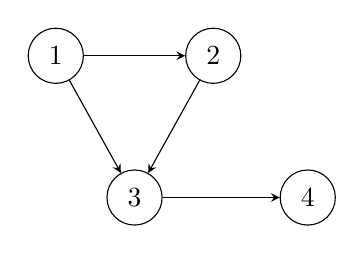
\begin{tikzpicture}[>=stealth,every node/.style={circle,draw,minimum size=7mm}]
\node (1) at (0,0) {1}; \node (2) at (2,0) {2}; \node (3) at (1,-1.8) {3}; \node (4) at (3.2,-1.8) {4};
\draw[->] (1) -- (2); \draw[->] (2) -- (3); \draw[->] (3) -- (4); \draw[->] (1) -- (3);
\end{tikzpicture}
\end{center}
\end{column}
\end{columns}
\note{Week 12 per the topic map: Graphs and Network Reasoning: paths, connectivity, traversal, shortest path, with the question of solving the graph correctly vs modeling reality incorrectly. The edge meaning must stay explicit. Tie-back: today's dice triangle and prerequisite cycle are already graph questions. Exit routine: collect the boundary sentence and the first-vs-current confidence number as the exit ticket. Remind students about Checkpoint 2.}
\end{frame}

\end{document}
